\section{AC-analysis}
AC-analysis and simulations where done with the following simulation setup.
\begin{figure}[!htbp]
    \centering
    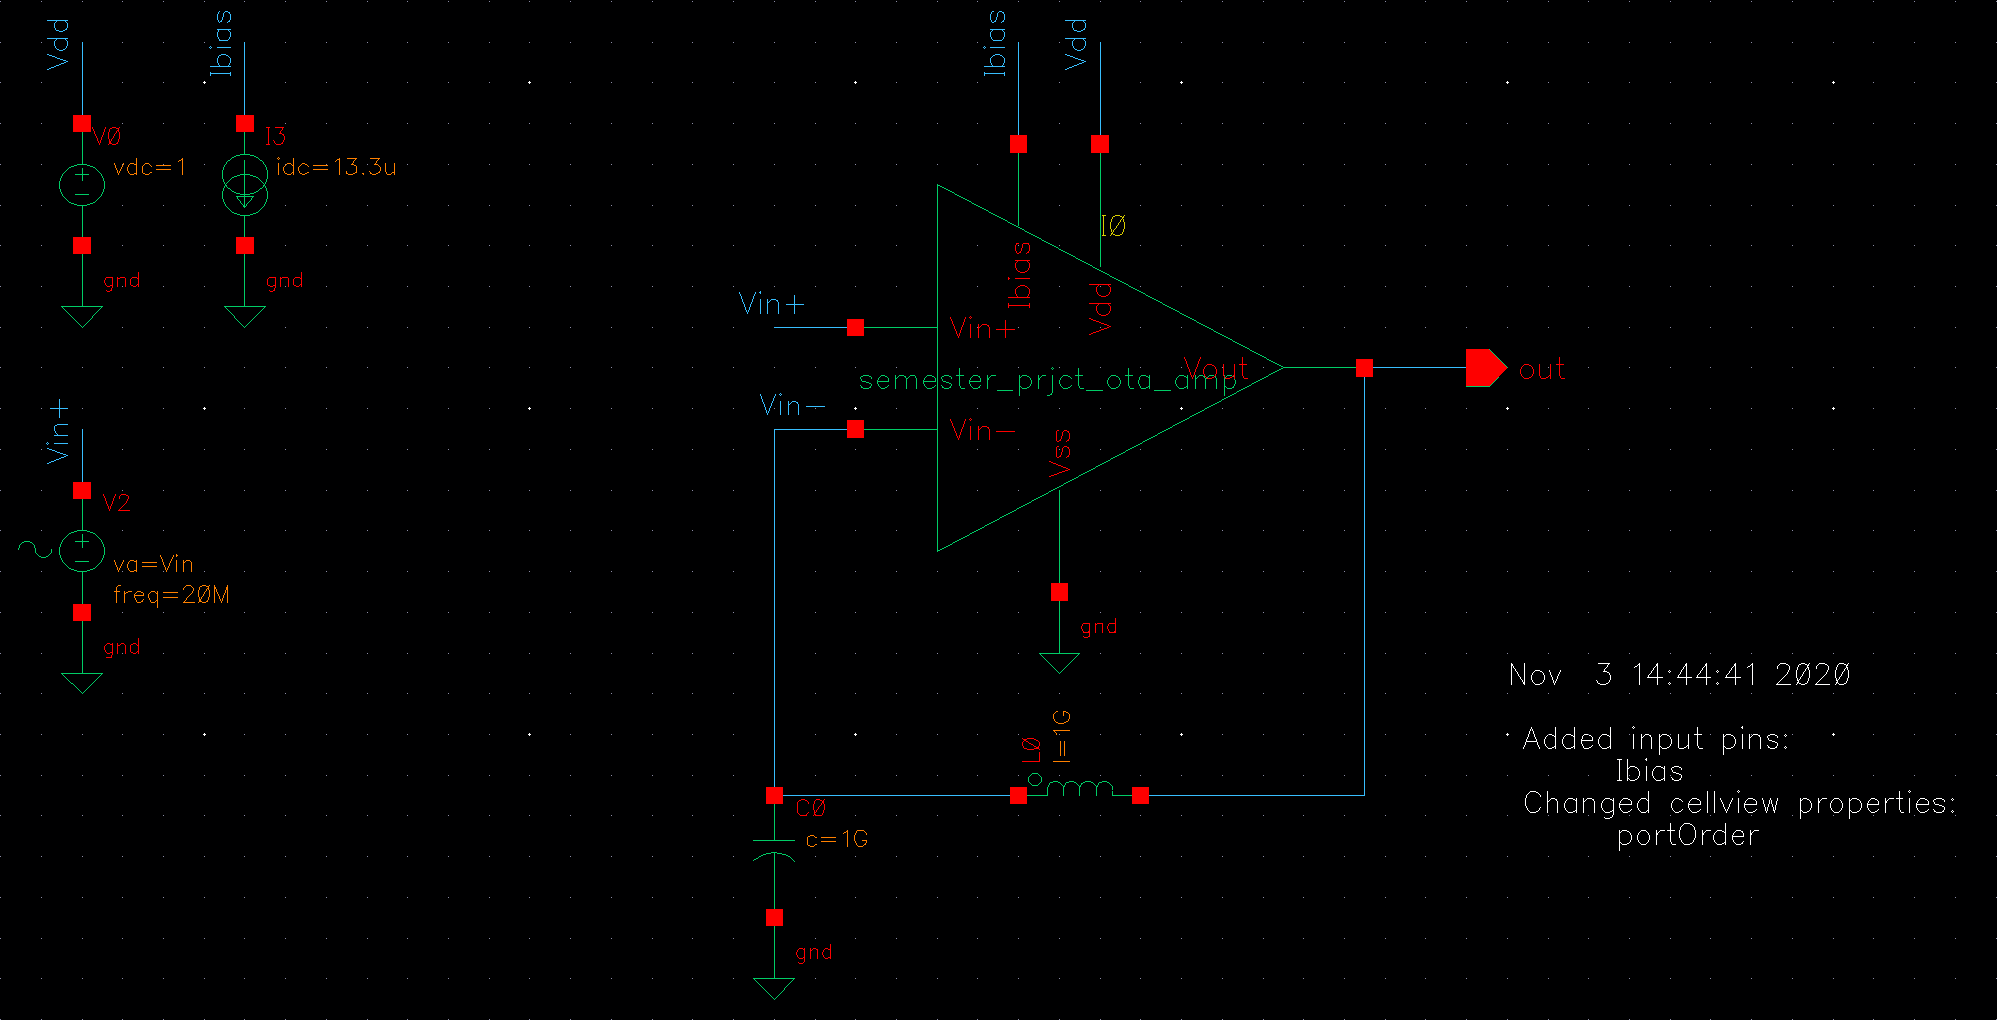
\includegraphics[width=.9\linewidth]{Images/Virtuoso/AC_tb.png}
    \caption{AC testbench}
    \label{fig:AC:tb}
\end{figure}
\begin{figure}[ht]
    \centering
    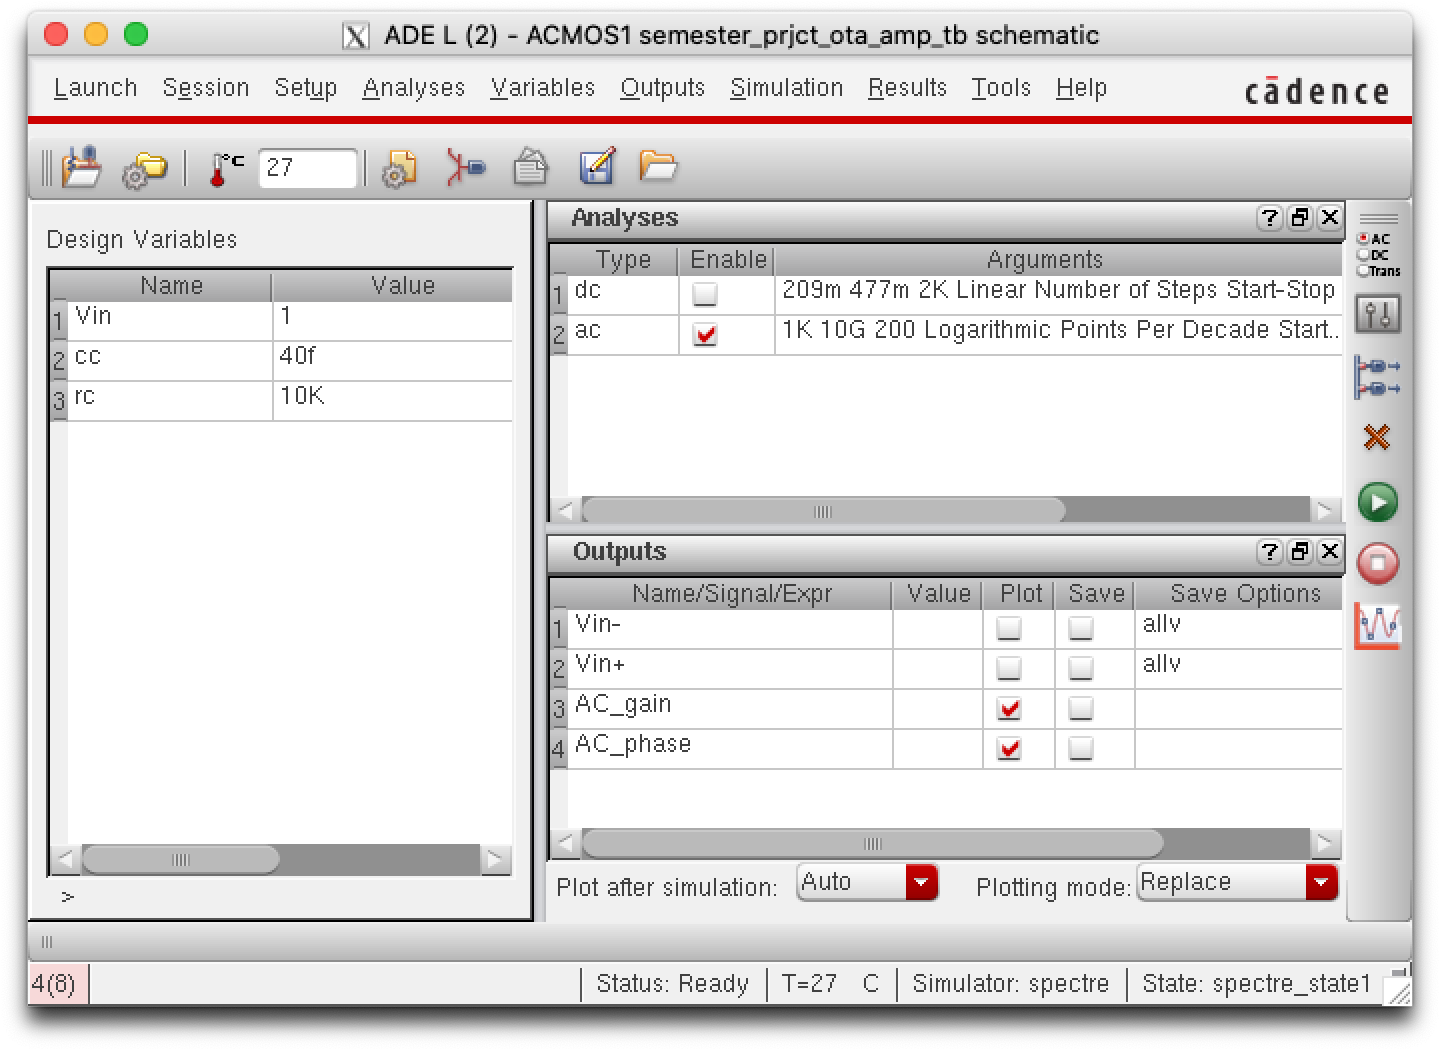
\includegraphics[width=.9\linewidth]{Images/Virtuoso/AC_stimuli.png}
    \caption{ADE L setup for AC analysis}
    \label{fig:ADE:AC}
\end{figure}

Had to add compensation components, started with $C_{c}$ = \SI{50}{\femto\farad} \& $R_{C}$ = \SI{10}{\kilo\ohm}. After some tweaking the values where changed to $C_{c}$ = \SI{40}{\femto\farad} and $R_{C}$, as this creates a decent phasemargin while still maintaining a decent gain, as seen in figure \ref{fig:AC:sim} and figure \ref{fig:AC:sim:z:phase}.
\newpage
\null
\vfill
\begin{figure}[H]
    \centering
    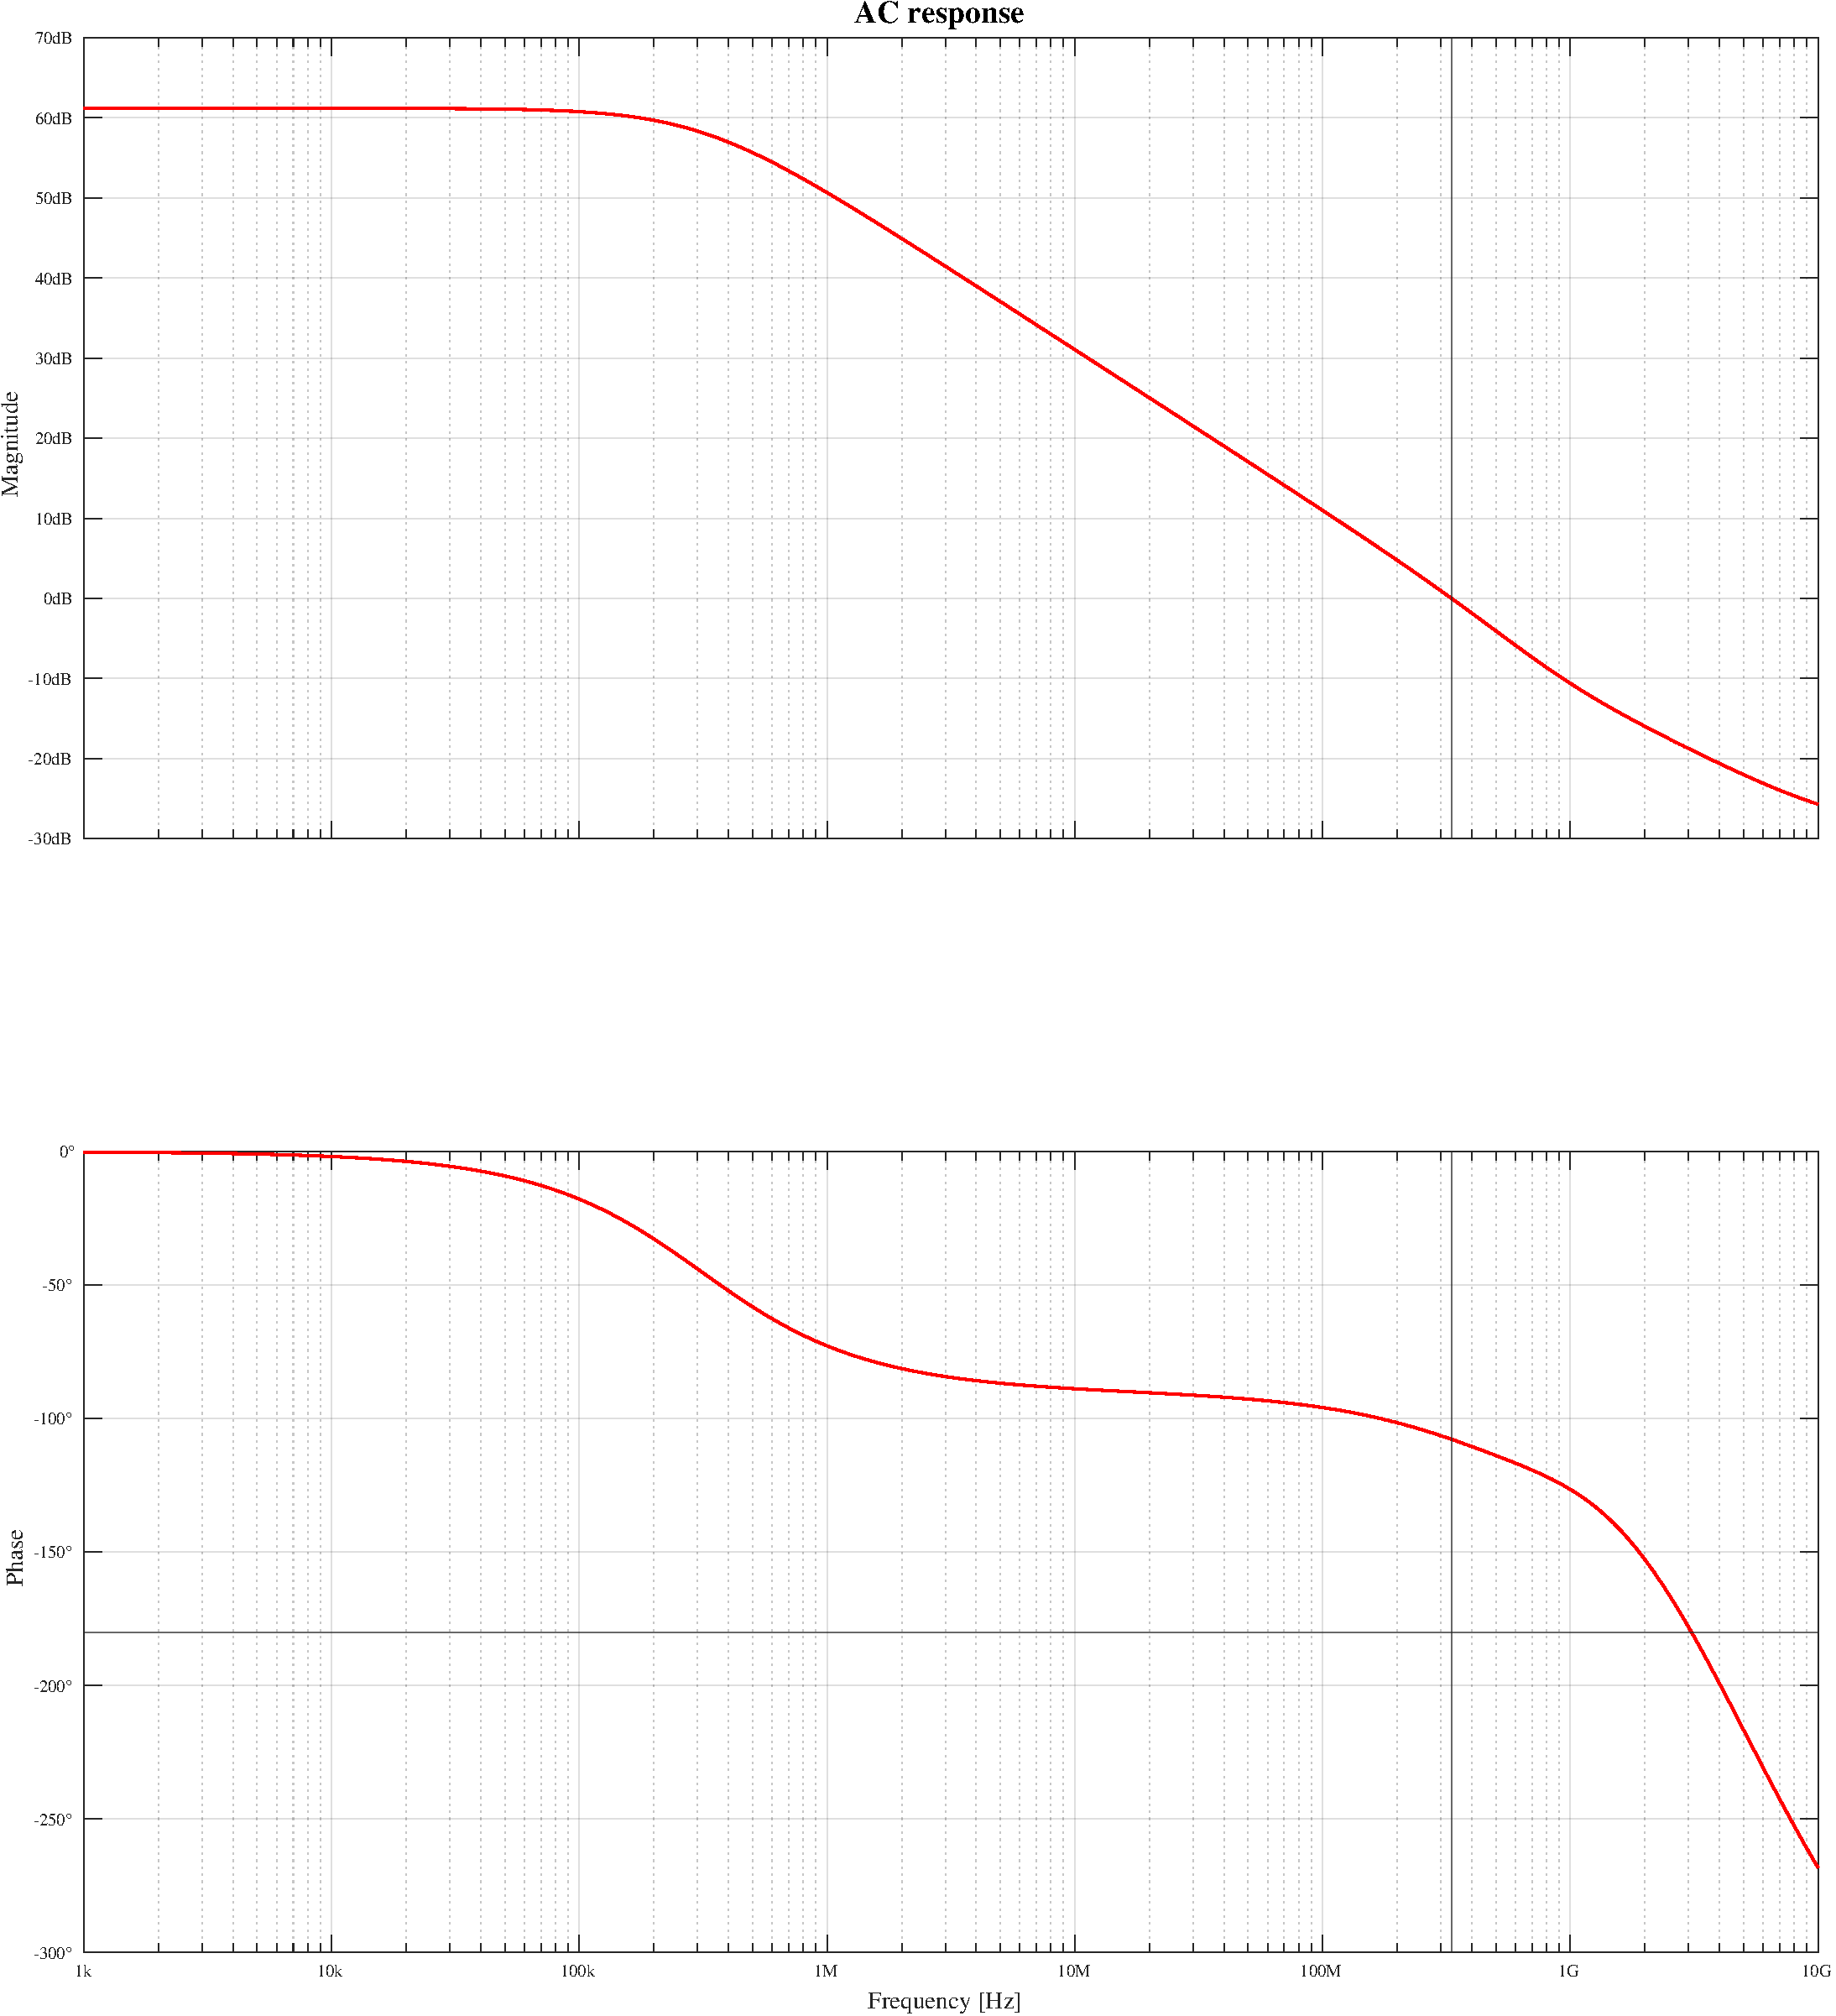
\includegraphics[width=.9\linewidth]{Images/Simulations/ac_response.pdf}
    \caption{AC (open-loop) response with $C_{C}$ = \SI{40}{\femto\farad} and $R_{C}$ = \SI{10}{\kilo\ohm}}
    \label{fig:AC:sim}
\end{figure}

\vfill
\newpage
\null
\vfill
\begin{figure}[H]
    \centering
    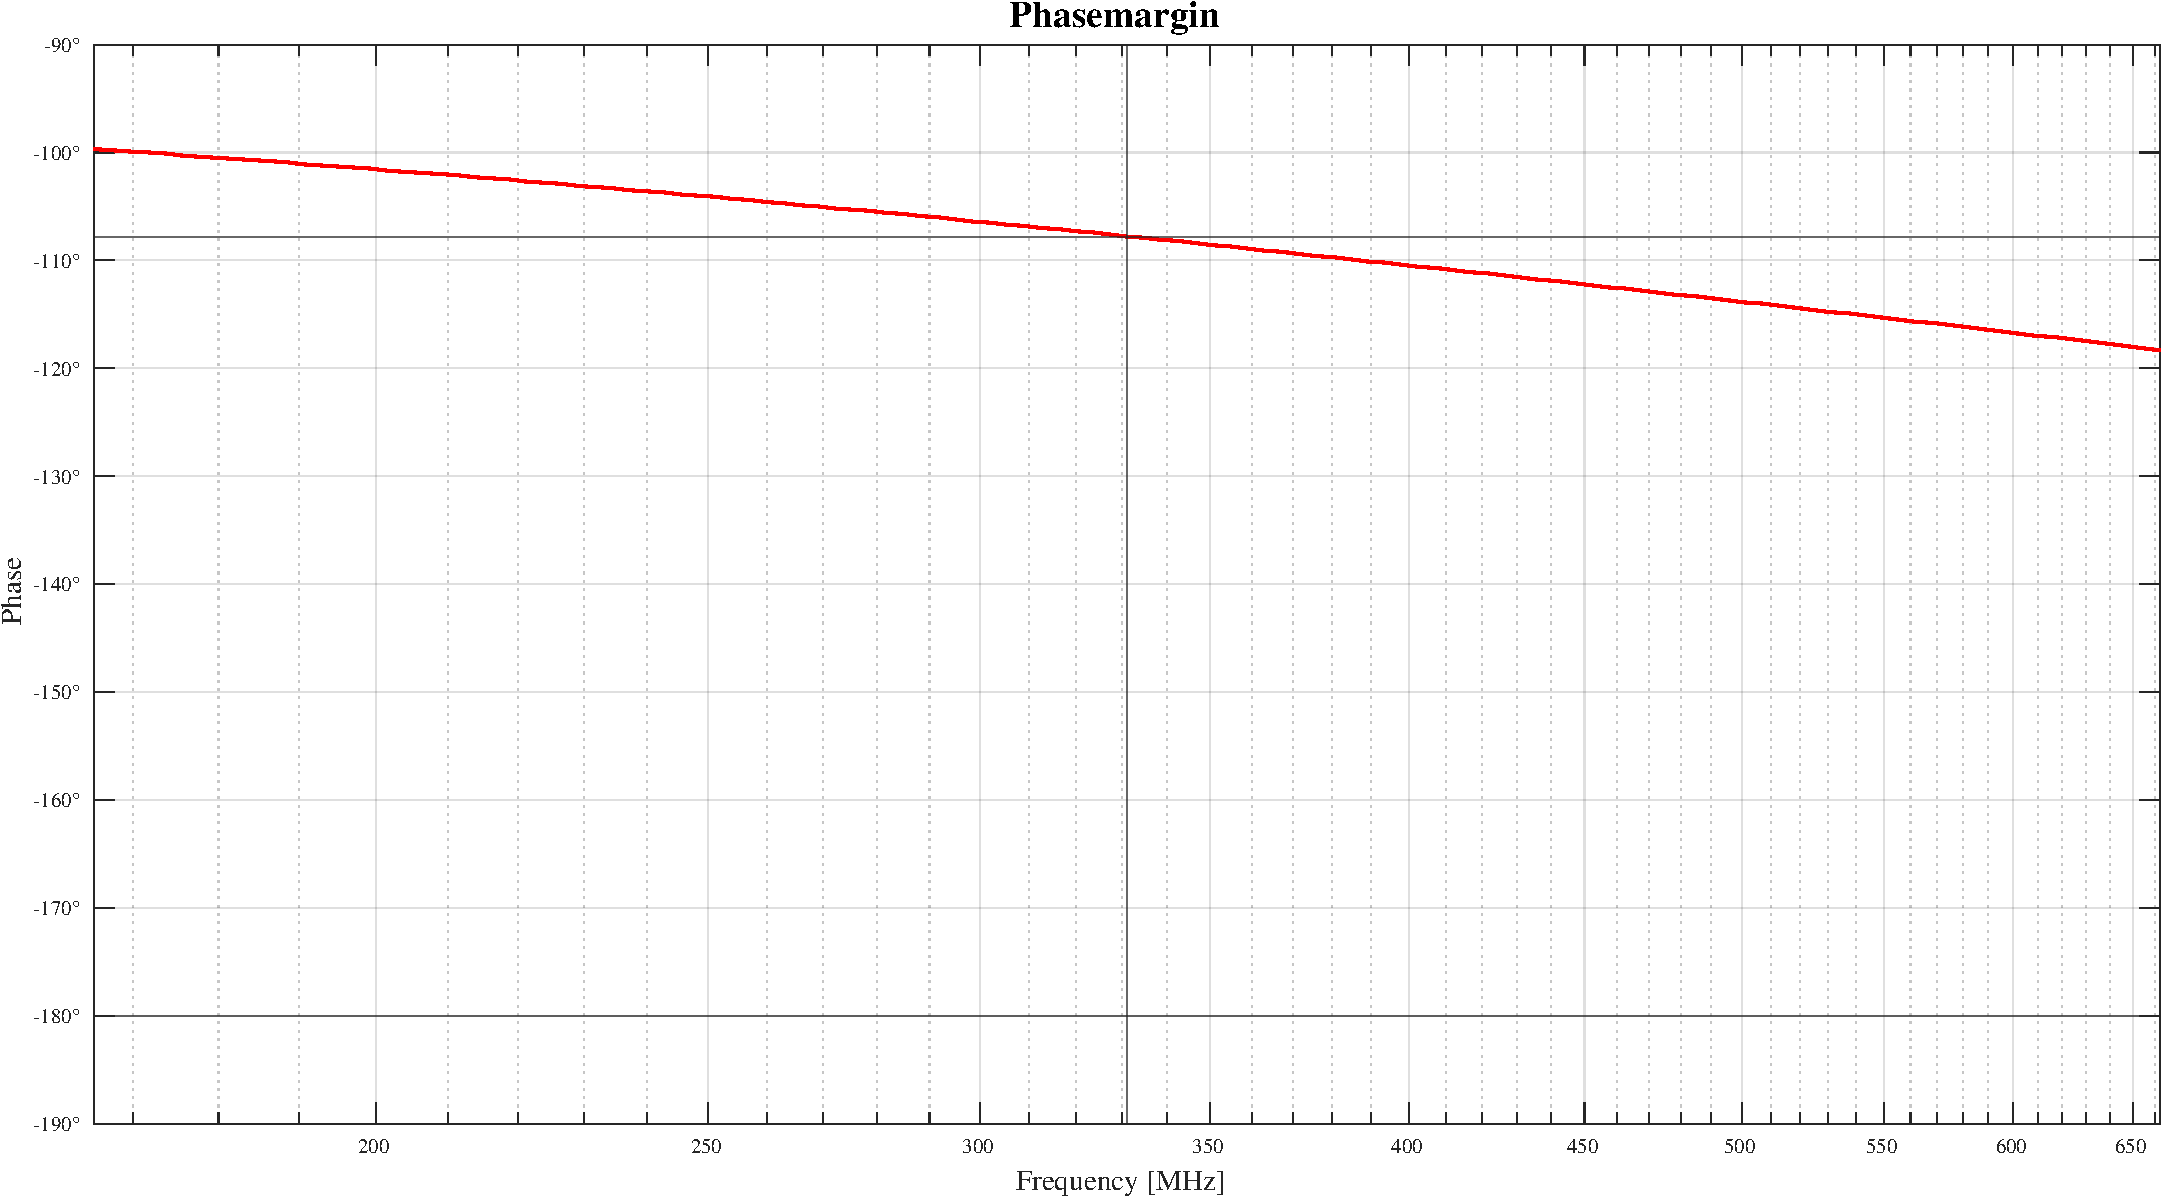
\includegraphics[width=.87\linewidth]{Images/Simulations/zoomed_phase_margin.pdf}
    \caption{Phase margin with $C_{C}$ = \SI{40}{\femto\farad} and $R_{C}$ = \SI{10}{\kilo\ohm}}
    \label{fig:AC:sim:z:phase}
\end{figure}
\vfill

\newpage
\null
\vfill
\begin{figure}[H]
    \centering
    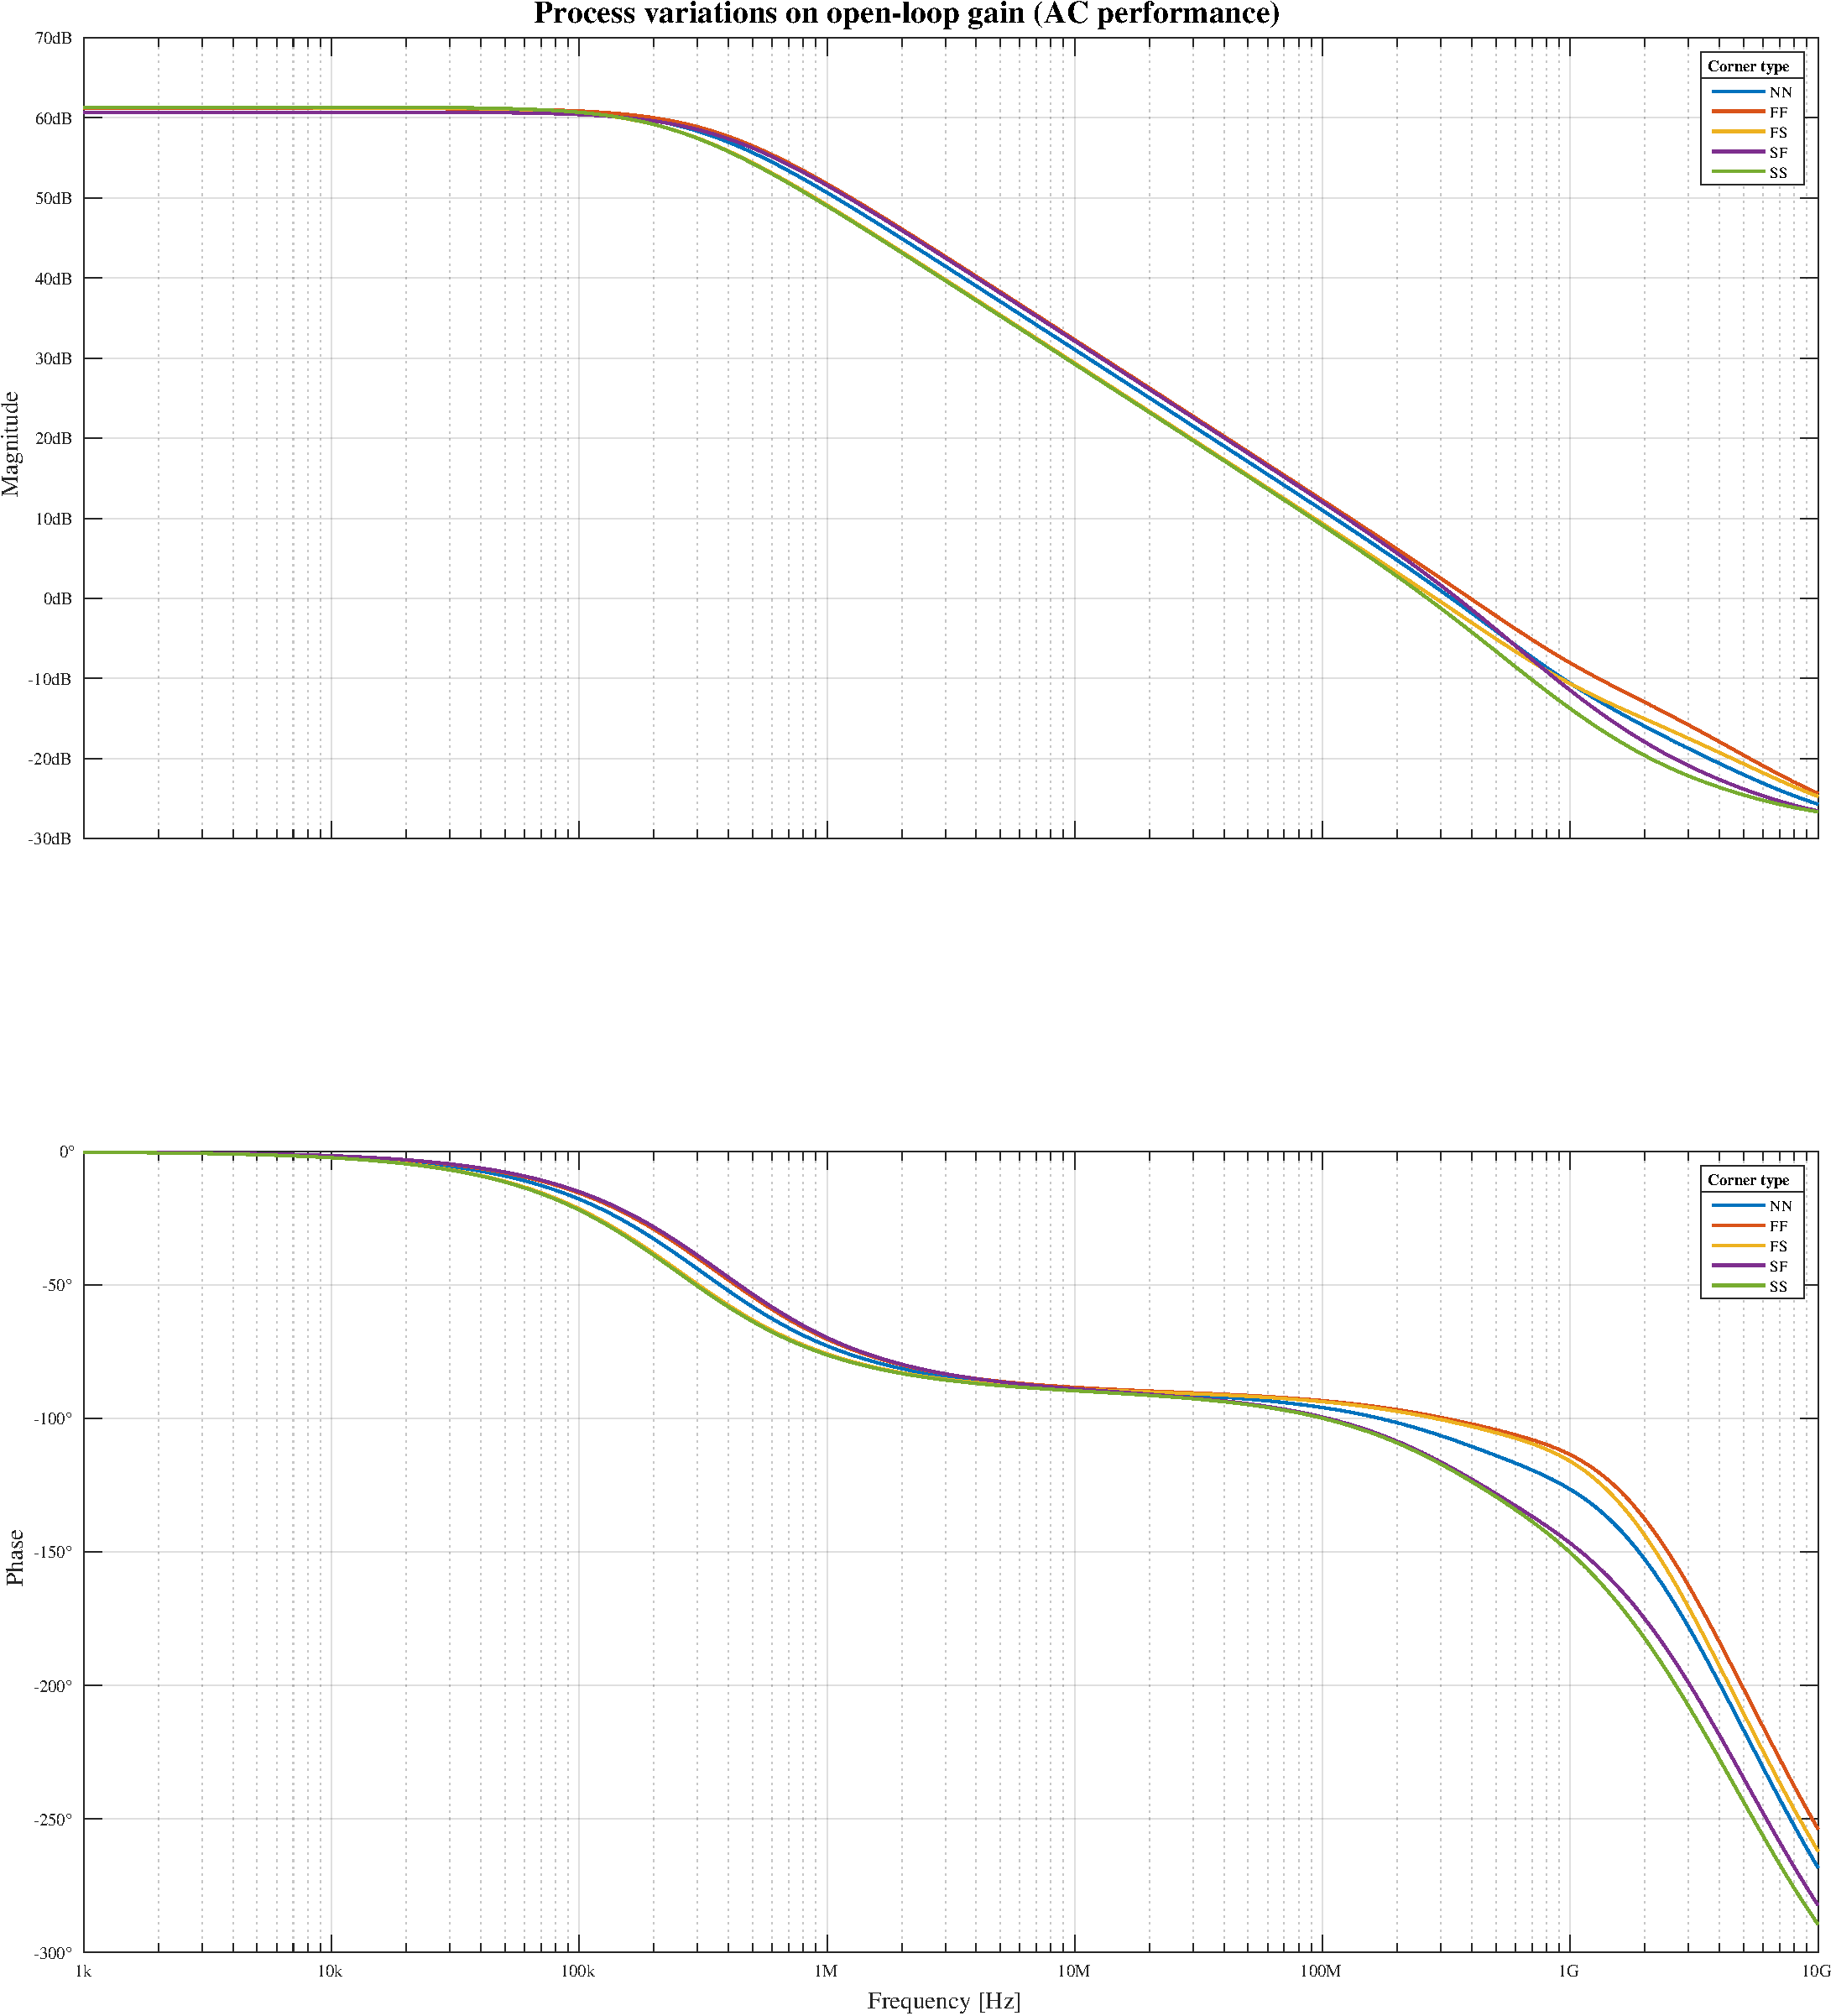
\includegraphics[width=1\linewidth]{Images/Simulations/corneranalysis.pdf}
    \caption{Process variations}
    \label{fig:process:variations:sim}
\end{figure}
\vfill